\subsubsection{Przykład}
\begin{figure}[h]
	\centering
	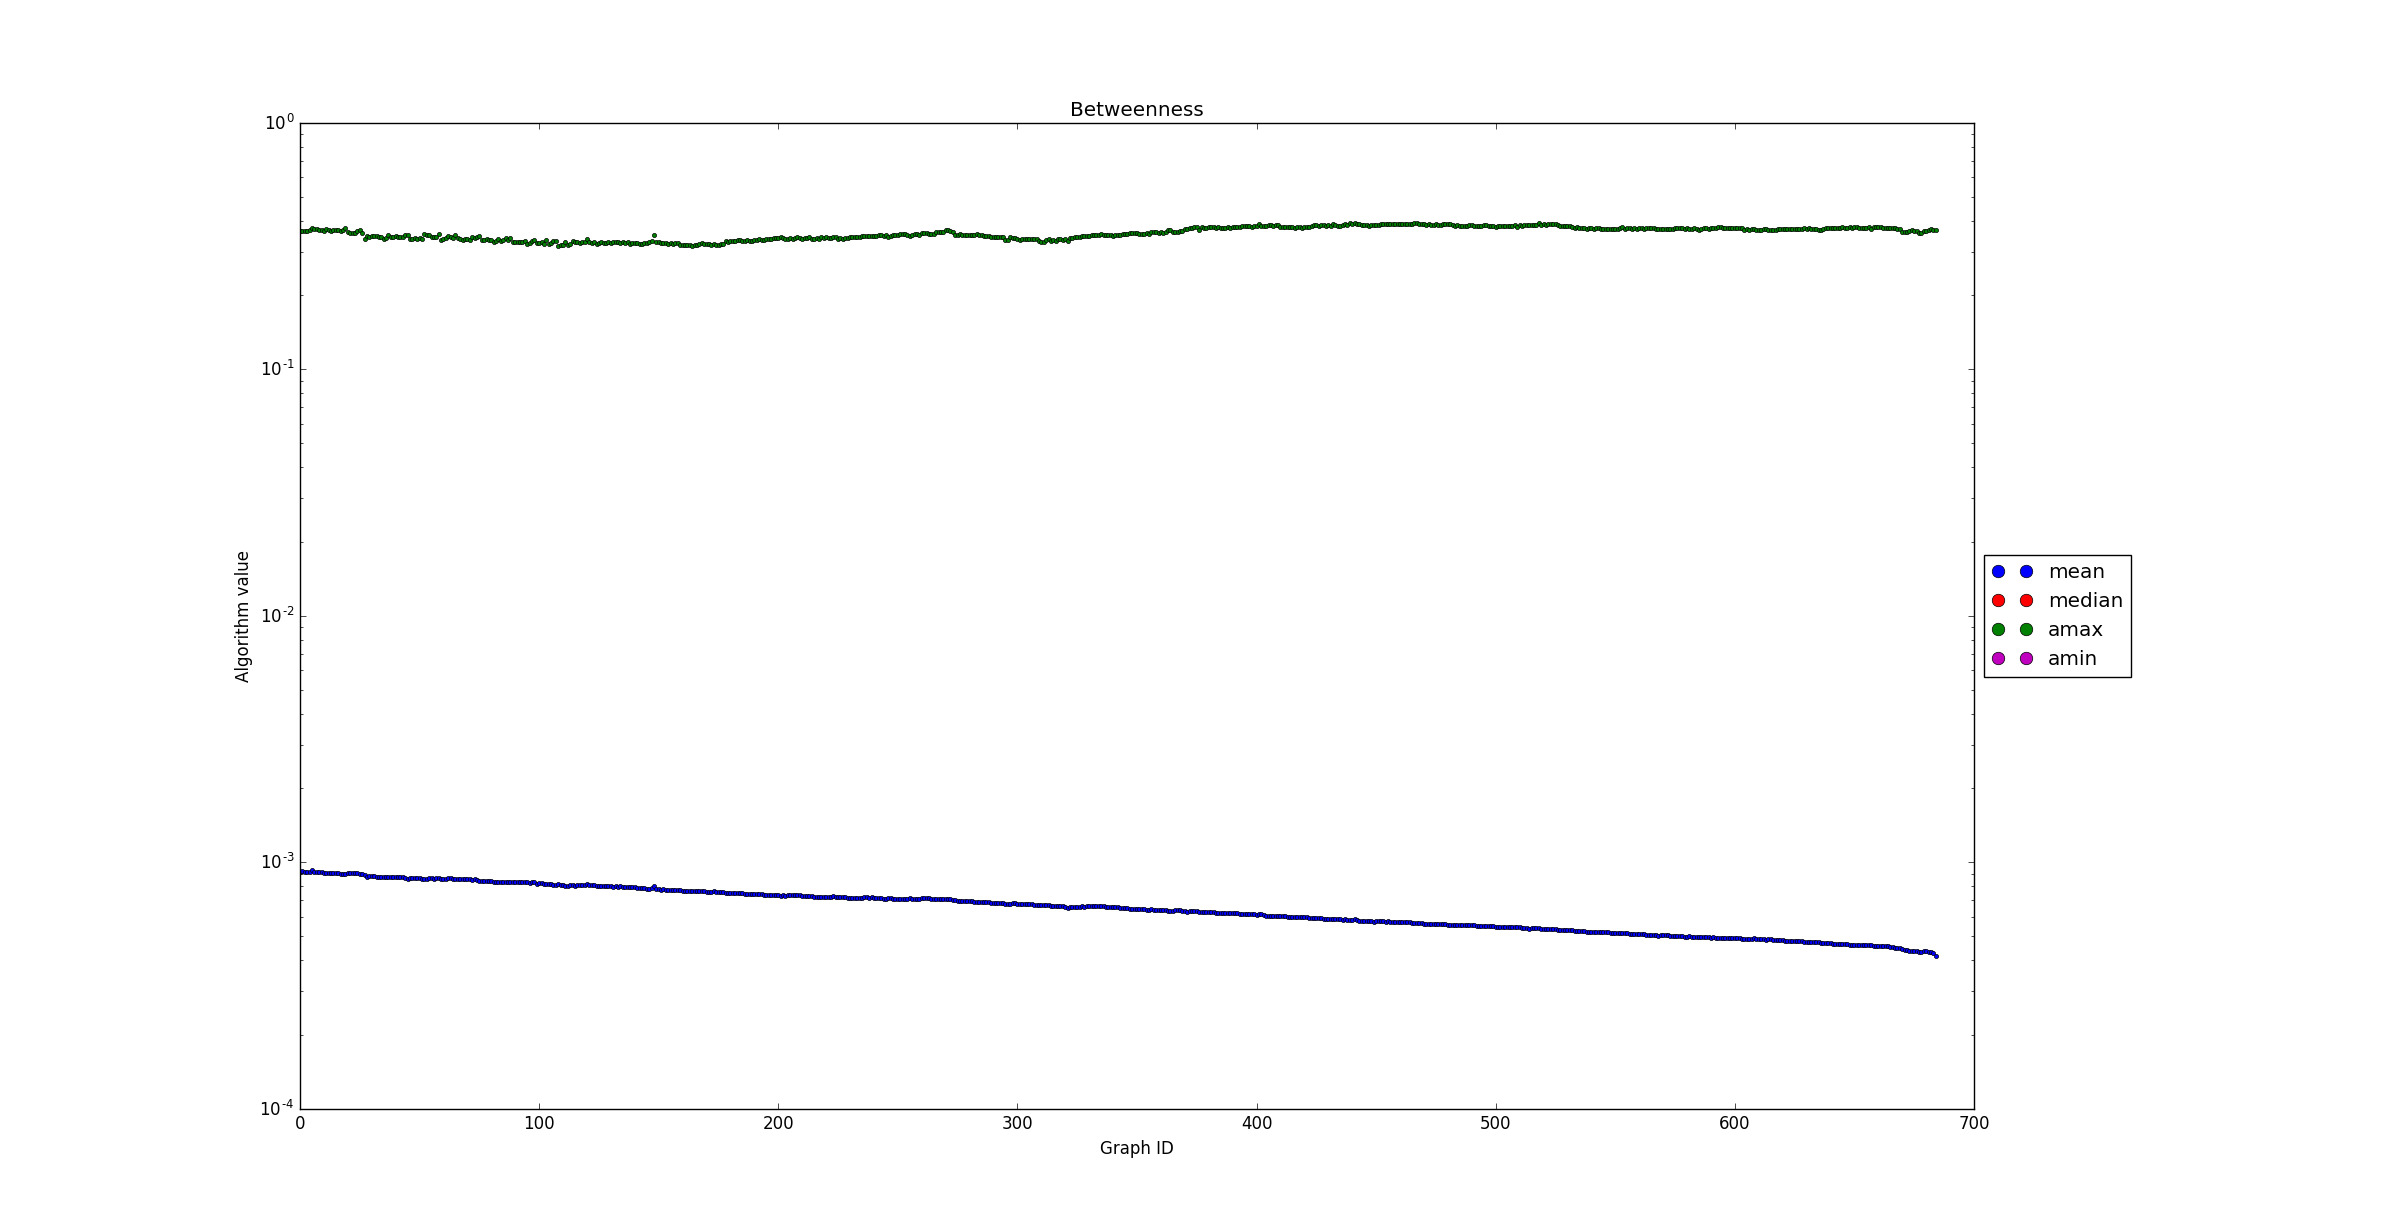
\includegraphics[width=\textwidth]{betweenness}
	\caption{Działanie Betweenness Centrality  na przykładowym grafie}
\end{figure}
\FloatBarrier
\subsubsection{Przykład}
\begin{figure}[h]
	\centering
	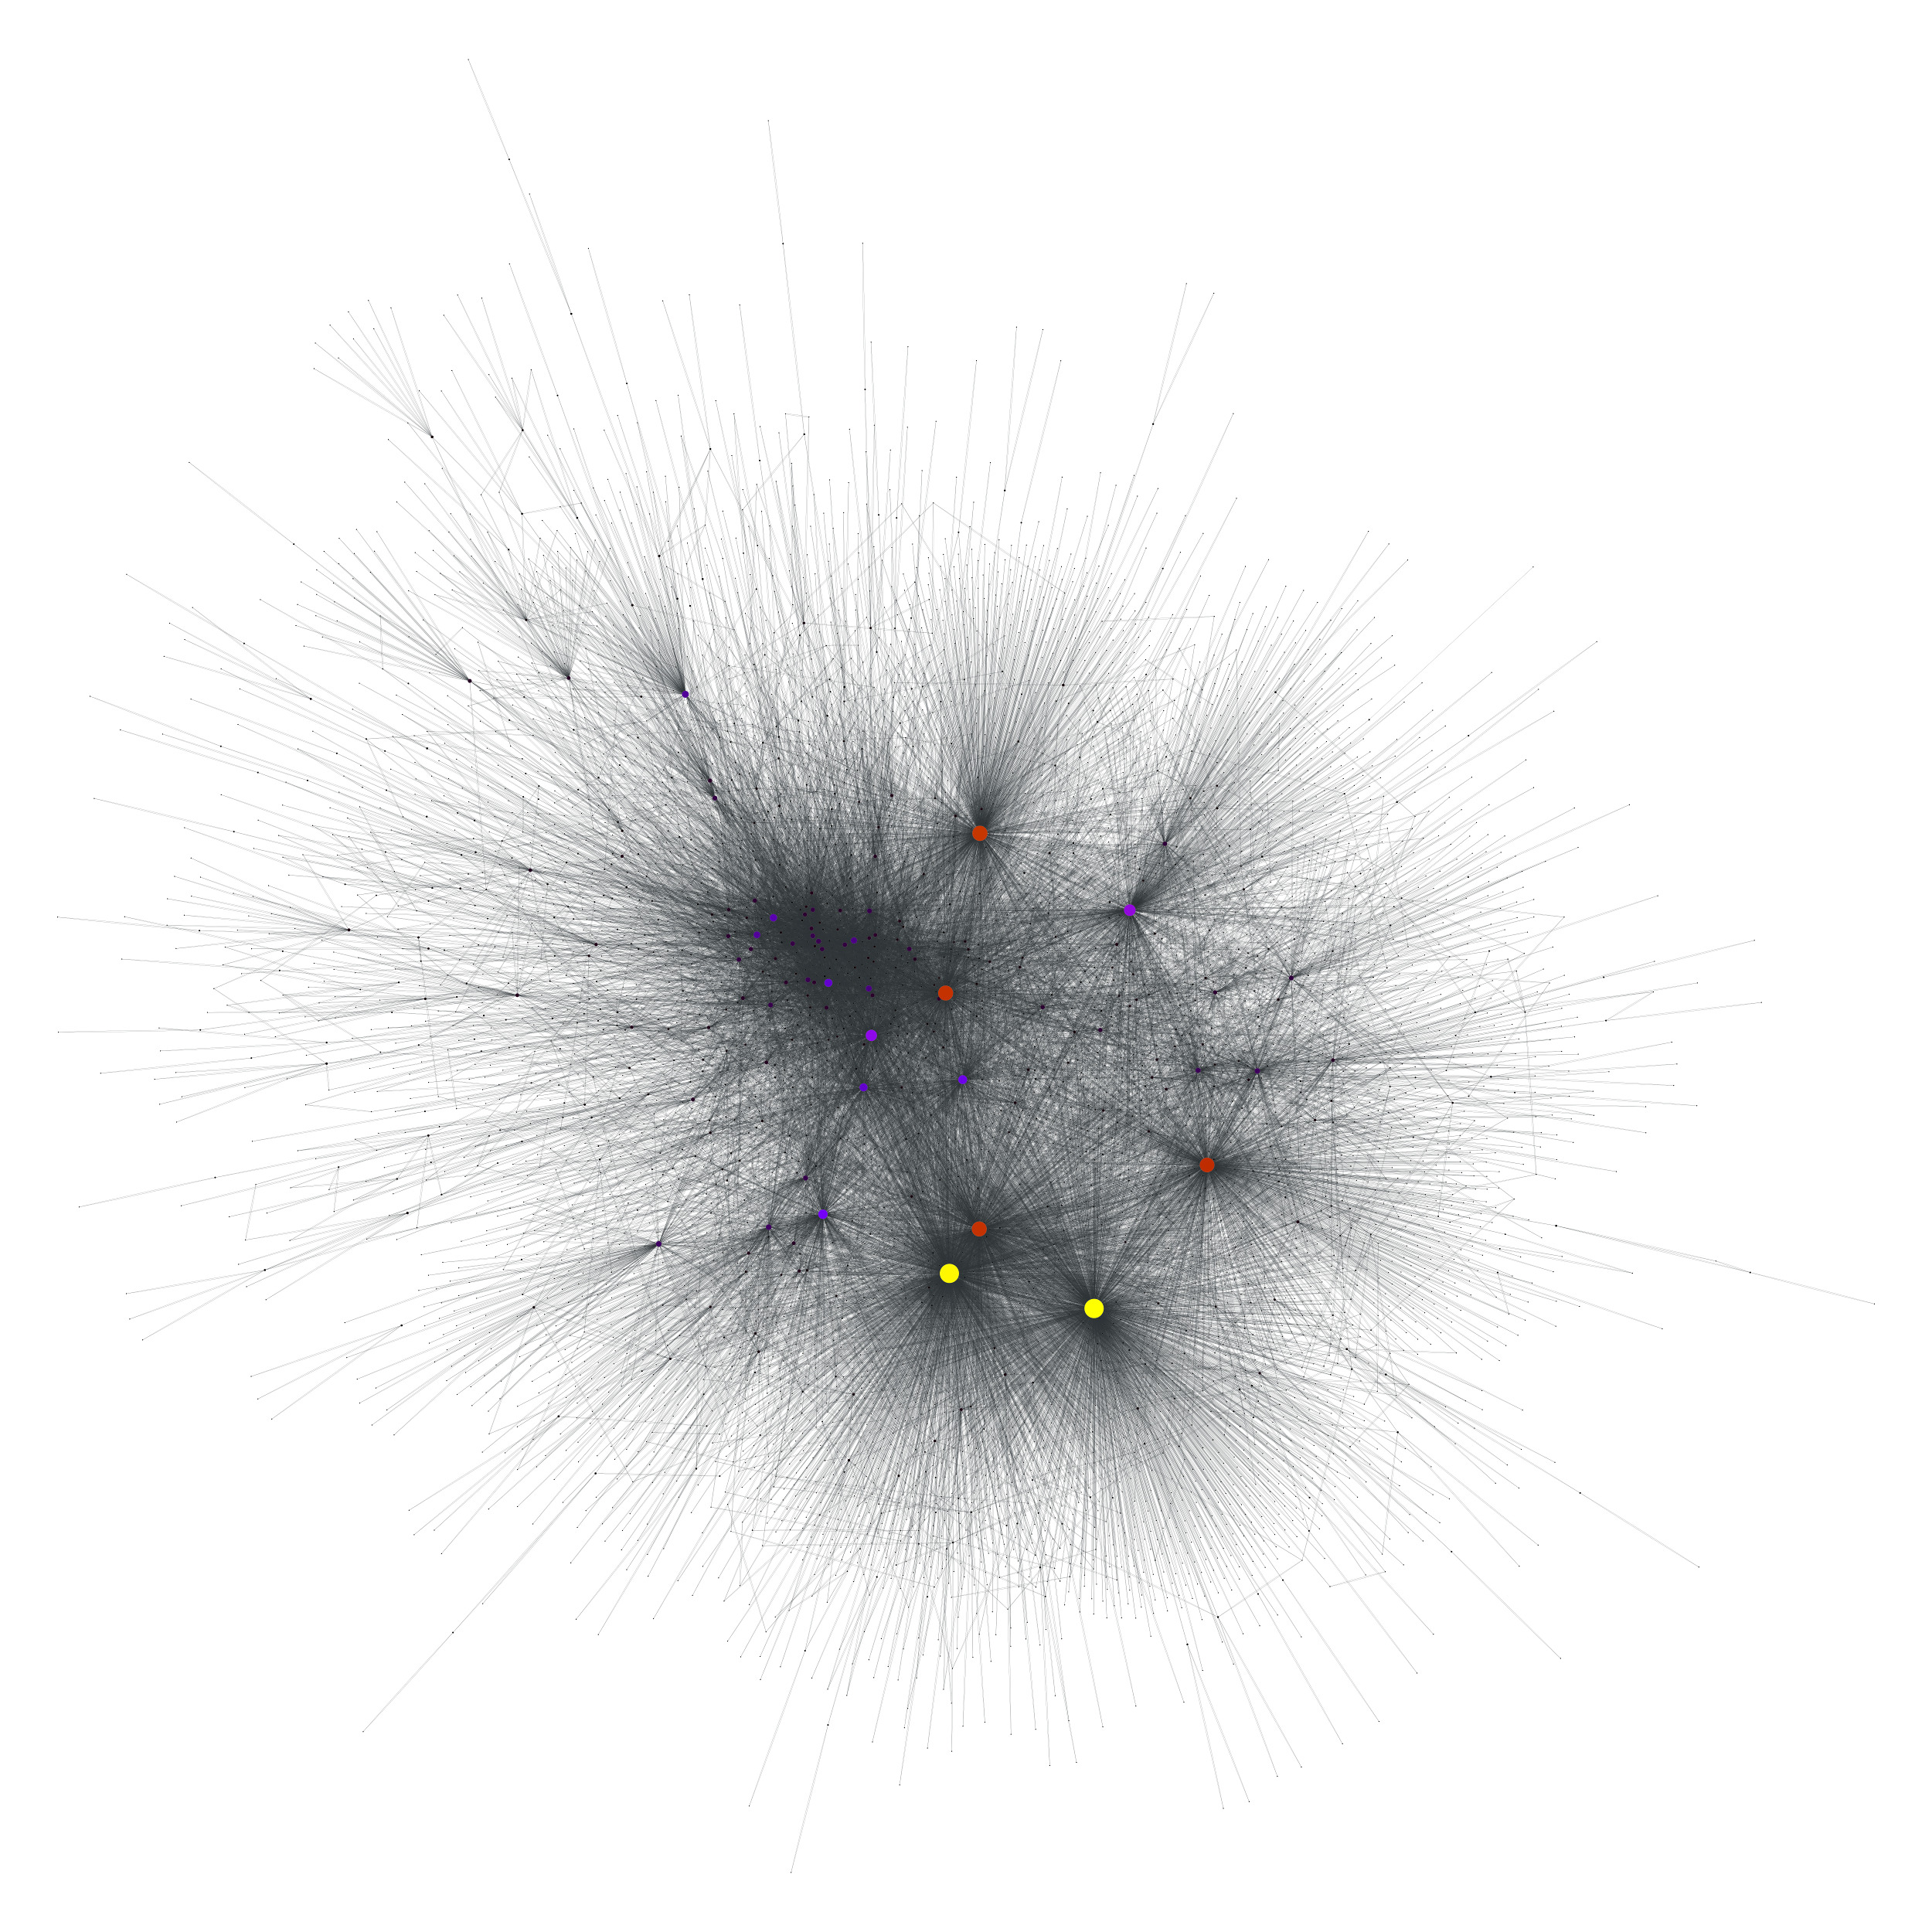
\includegraphics[width=\textwidth]{betweenness_8k}
	\caption{Działanie Betweenness Centrality  na przykładowym grafie}
\end{figure}
\FloatBarrier
\subsubsection{Przykład}
\begin{figure}[h]
	\centering
	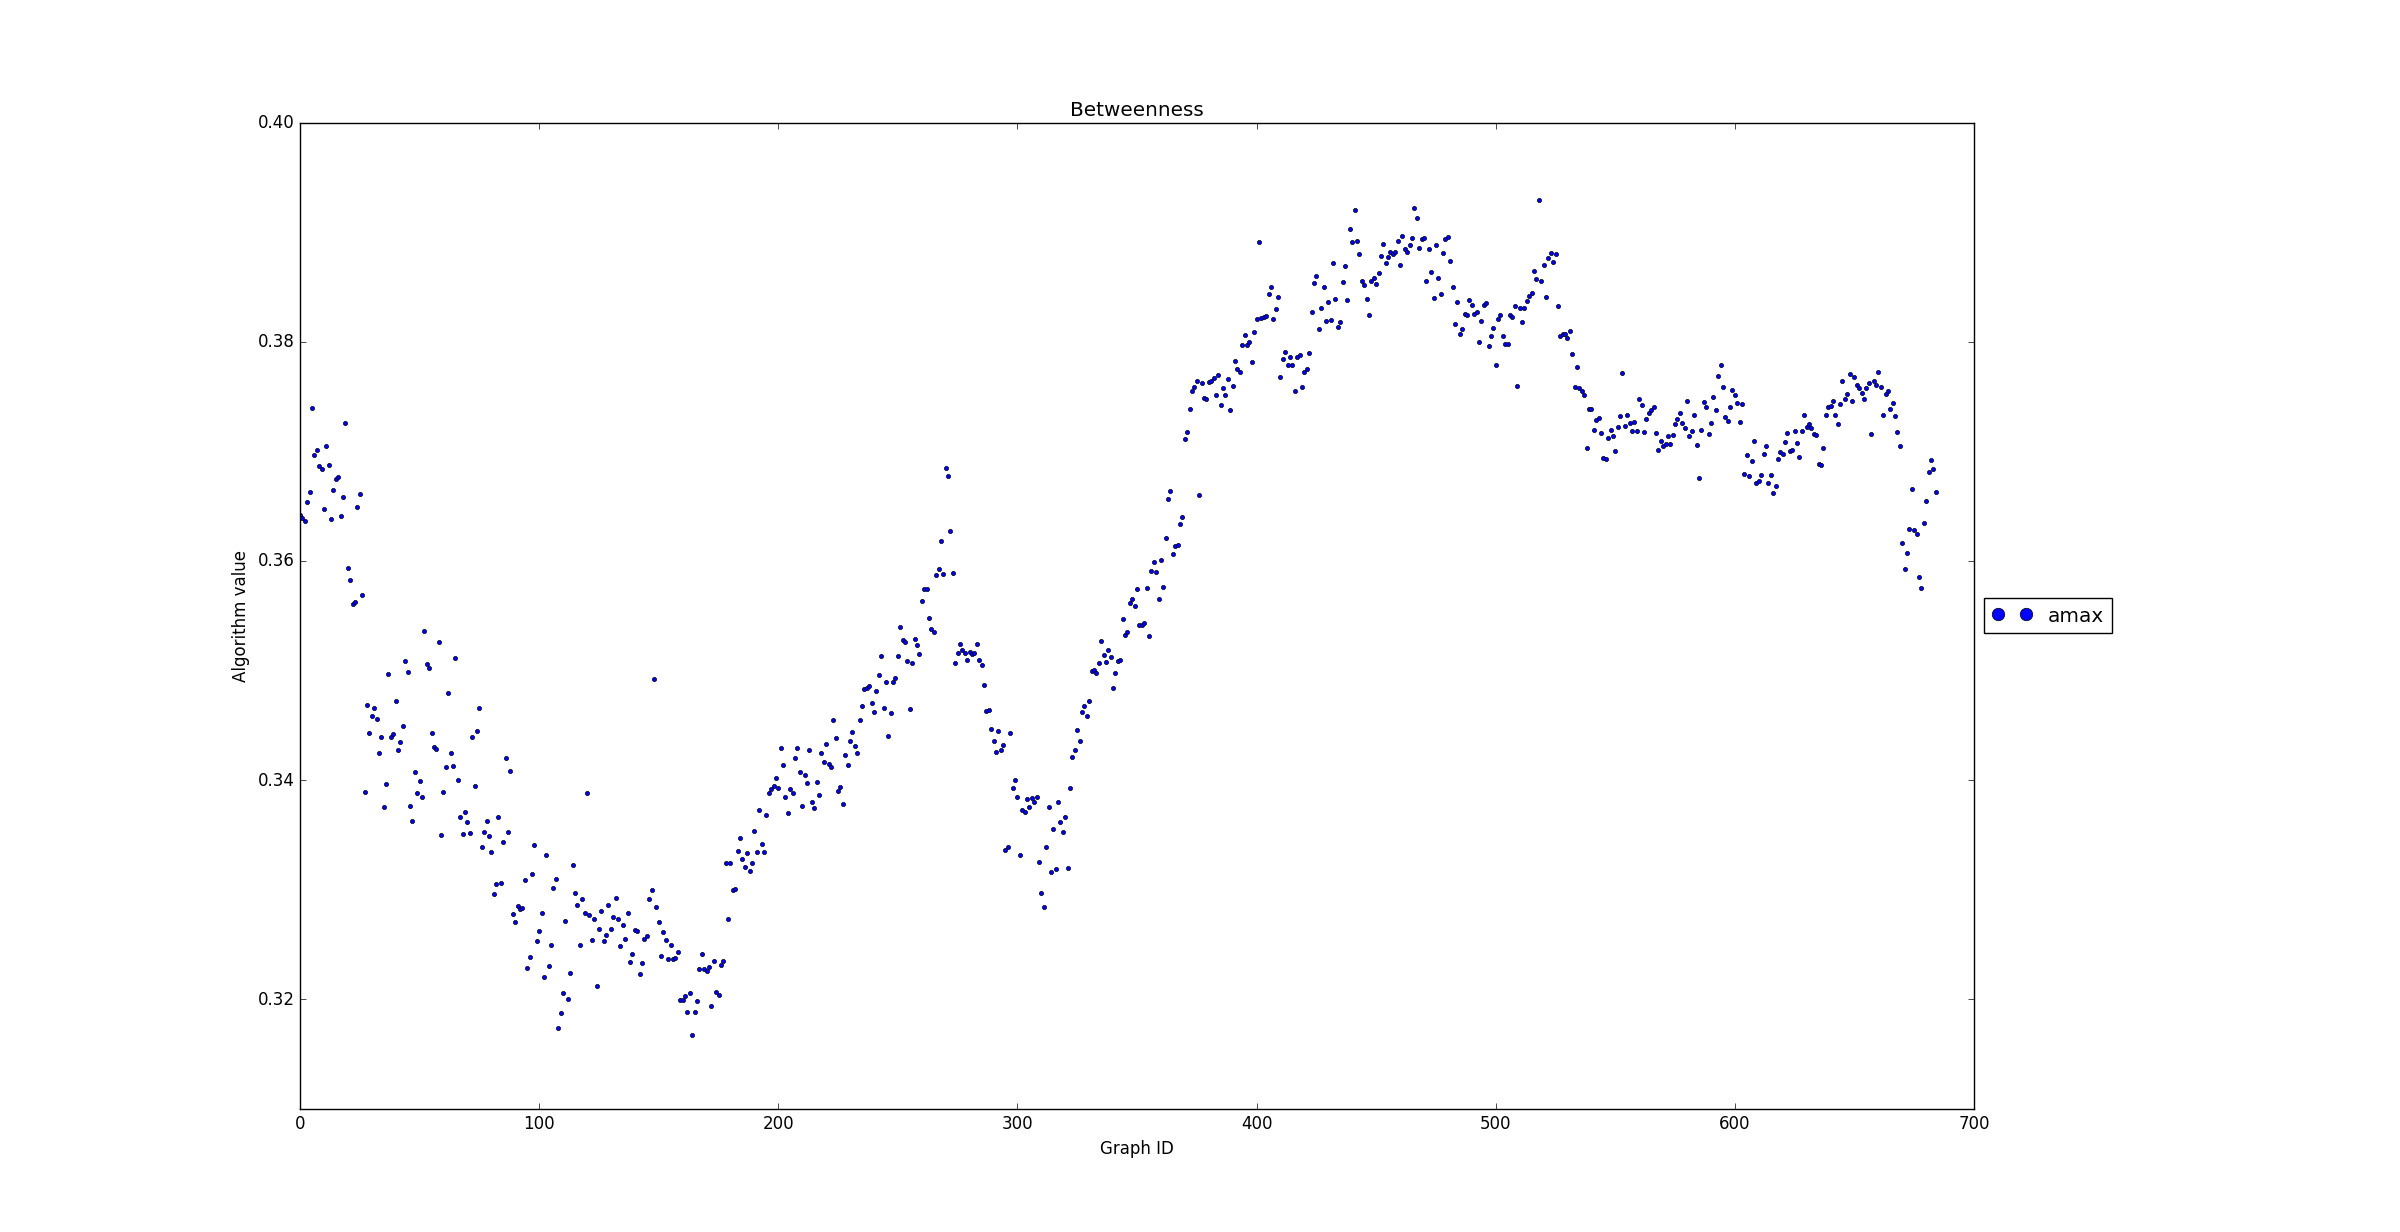
\includegraphics[width=\textwidth]{betweenness_max}
	\caption{Działanie Betweenness Centrality  na przykładowym grafie}
\end{figure}
\FloatBarrier\FloatBarrier
\subsubsection{Przykład}
\begin{figure}[h]
	\centering
	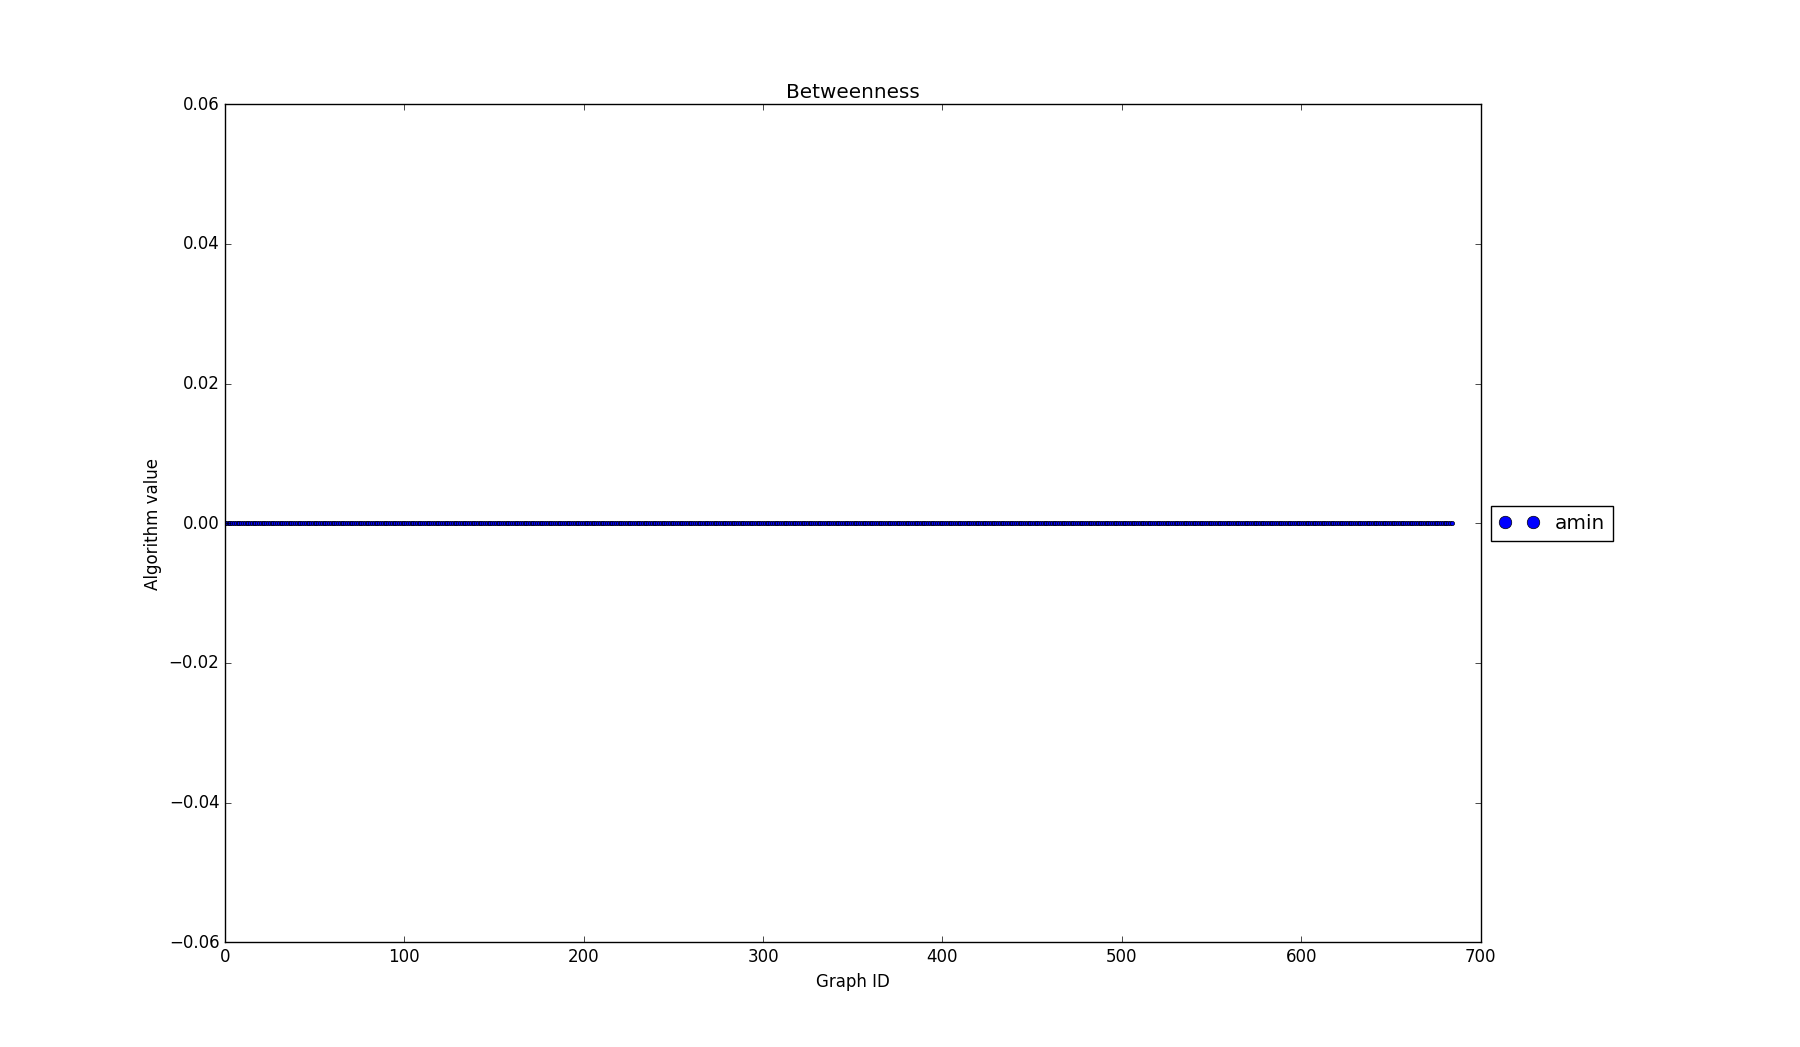
\includegraphics[width=\textwidth]{betweenness_min}
	\caption{Działanie Betweenness Centrality  na przykładowym grafie}
\end{figure}
\FloatBarrier\FloatBarrier
\subsubsection{Przykład}
\begin{figure}[h]
	\centering
	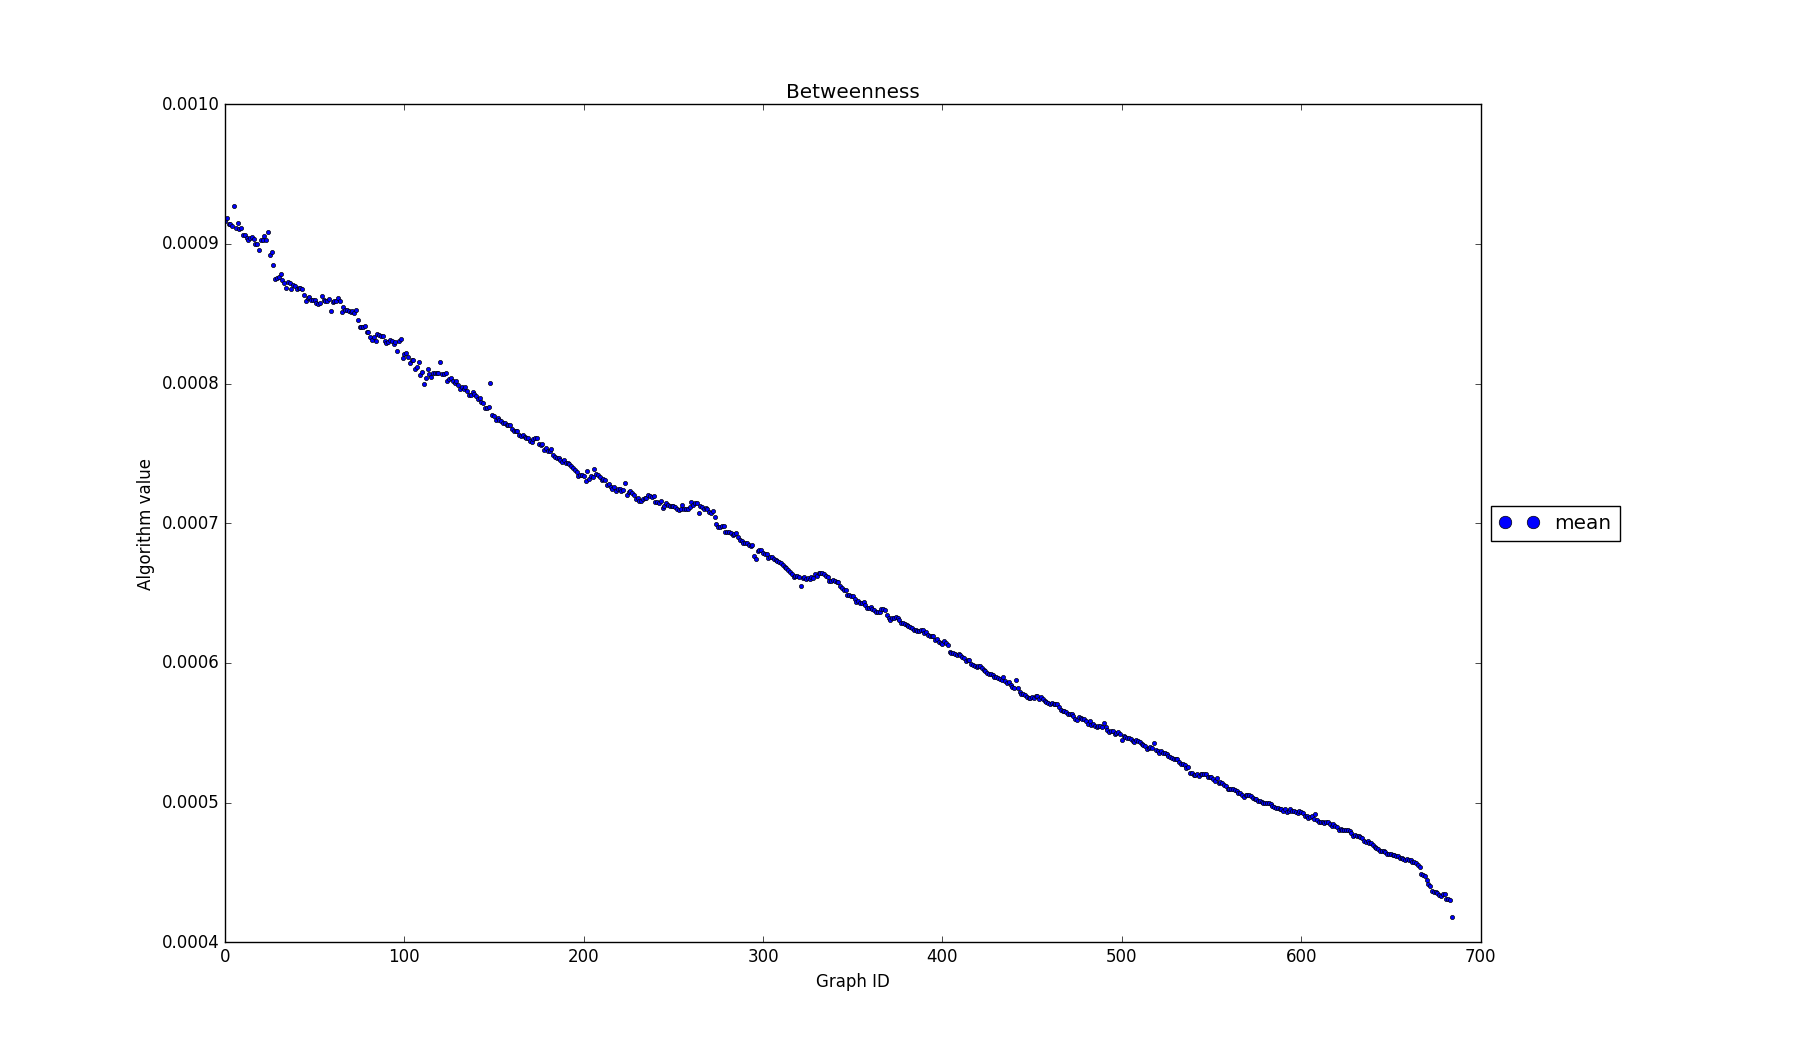
\includegraphics[width=\textwidth]{betweenness_mean}
	\caption{Działanie Betweenness Centrality  na przykładowym grafie}
\end{figure}
\FloatBarrier\FloatBarrier
\subsubsection{Przykład}
\begin{figure}[h]
	\centering
	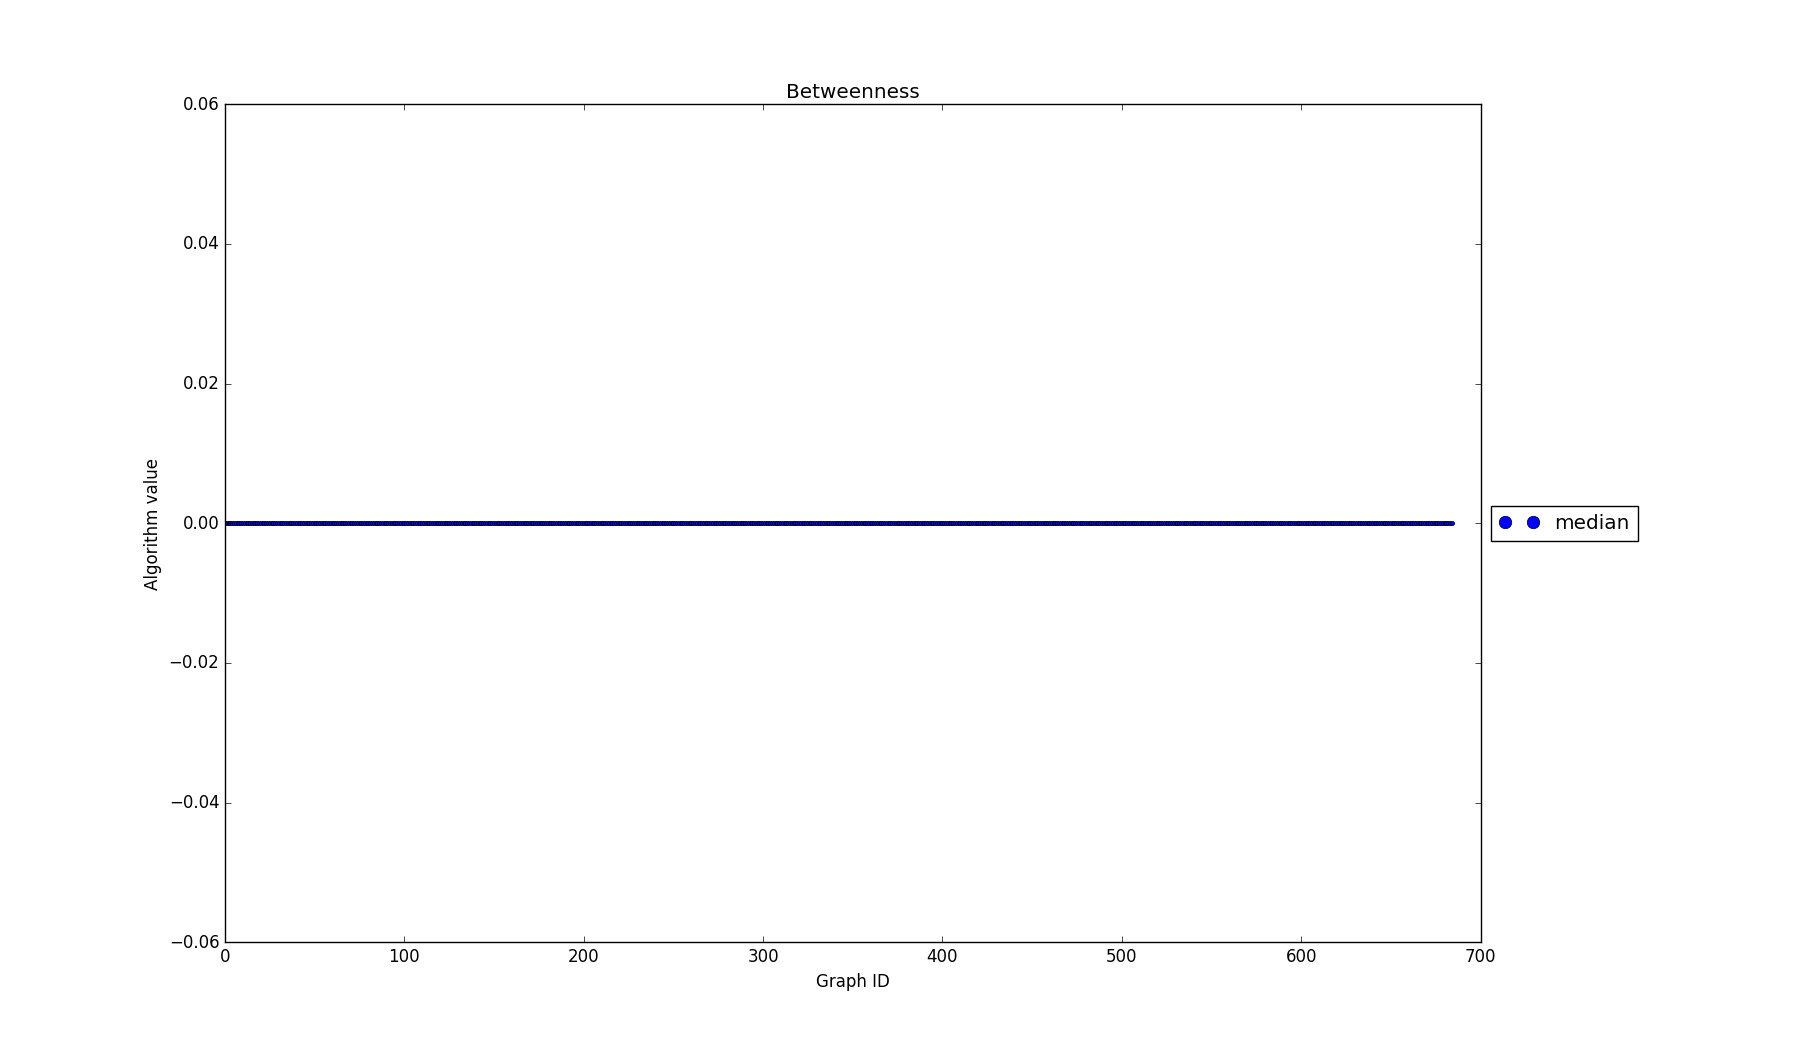
\includegraphics[width=\textwidth]{betweenness_median}
	\caption{Działanie Betweenness Centrality  na przykładowym grafie}
\end{figure}
\FloatBarrier